\documentclass[a4paper]{jpconf}

\usepackage{graphicx}
\usepackage{bm}        % for math
\usepackage{amssymb}   % for math
\usepackage{amsfonts}
\usepackage{amsmath}
\usepackage{epsfig}
\usepackage{units}
\usepackage{cite}
%\usepackage[numbers,square,sort&compress]{natbib}
\usepackage[utf8]{inputenc}
\usepackage[T1]{fontenc}
\usepackage{color}
\usepackage{hyperref}
\usepackage{lineno}
\linenumbers

%particles
\newcommand{\jpsi}{\rm J/$\psi$}
\newcommand{\psip}{$\psi^\prime$}
\newcommand{\jpsiDY}{\rm J/$\psi$\,/\,DY}
\newcommand{\chic}{$\chi_{\rm c}$}
\newcommand{\pip}{$\pi^{+}$}
\newcommand{\pim}{$\pi^{-}$}
\newcommand{\pizero}{$\pi^{0}$}
\newcommand{\kap}{K$^{+}$}
\newcommand{\kam}{K$^{-}$}
\newcommand{\pbar}{$\rm\overline{p}$}
\newcommand{\ccbar}{\ensuremath{\mathrm{c\overline{c}}}}
\newcommand{\bbbar}{\ensuremath{\mathrm{b\overline{b}}}}
\newcommand{\Dzero}{\ensuremath{\mathrm{D^{0}}}}
\newcommand{\Dzerobar}{\ensuremath{\mathrm{\overline{D}^{0}}}}
\newcommand{\Dpm}{\ensuremath{\mathrm{D^{\pm}}}}
\newcommand{\Ds}{\ensuremath{\mathrm{D_{s}^{\pm}}}}
\newcommand{\Dstar}{\ensuremath{\mathrm{D^{*\pm}}}}

%collision systems
\newcommand{\pp}{pp}
\newcommand{\pPb}{p--Pb}
\newcommand{\PbPb}{Pb--Pb}

%detectors
\newcommand{\ezdc}{$E_{\rm ZDC}$}

%units
\newcommand{\GeVc}{GeV/$c$}
\newcommand{\GeVcsq}{GeV/$c^2$}

%others
\newcommand{\degree}{$^{\rm o}$}
\newcommand{\s}{\ensuremath{\sqrt{s}}}
\newcommand{\snn}{\ensuremath{\sqrt{s_{\rm NN}}}}
\newcommand{\y}{\ensuremath{y}}
\newcommand{\pt}{\ensuremath{p_{\rm T}}}
\newcommand{\dedx}{d$E$/d$x$}
\newcommand{\dndy}{d$N$/d$y$}
\newcommand{\dndydpt}{${\rm d}^2N/({\rm d}y {\rm d}p_{\rm t})$}
\newcommand{\zpar}{\ensuremath{z_{||}}}
\newcommand{\zpargen}{\ensuremath{z_{||}^{\mathrm{part}}}}
\newcommand{\zpardet}{\ensuremath{z_{||}^{\mathrm{det}}}}
\newcommand{\ptchjet}{\ensuremath{p_{\mathrm{T,ch\, jet}}}}
\newcommand{\ptjet}{\ensuremath{p_{\mathrm{T,jet}}}}
\newcommand{\ptchjetgen}{\ensuremath{p_{\mathrm{T,ch\,jet}}^{\mathrm{part}}}}
\newcommand{\ptchjetdet}{\ensuremath{p_{\mathrm{T,ch\,jet}}^{\mathrm{det}}}}
\newcommand{\ptd}{\ensuremath{p_{\mathrm{T,D}}}}
\newcommand{\ptdgen}{\ensuremath{p_{\mathrm{T,D}}^{\mathrm{part}}}}
\newcommand{\ptddet}{\ensuremath{p_{\mathrm{T,D}}^{\mathrm{det}}}}
\newcommand{\antikt}{anti-\ensuremath{k_{\mathrm{T}}}}
\newcommand{\Antikt}{Anti-\ensuremath{k_{\mathrm{T}}}}
\newcommand{\kt}{\ensuremath{k_{\mathrm{T}}}}
\newcommand{\pthard}{\ensuremath{p_{\mathrm{T,hard}}}}

\begin{document}
\title{Measurement of D-meson tagged jets in pp collisions at 7 TeV with ALICE}

\author{Salvatore Aiola, for the ALICE Collaboration}

\address{Physics Department, Yale University, 266 Whitney Avenue, New Haven, CT 06511}

\ead{salvatore.aiola@cern.ch}

\begin{abstract}
We present the current status of the measurement of jets that contain a D meson (D-tagged jets) with \mbox{ALICE}.
D-meson candidates, identified via their hadronic decay channels, are combined with the other charged tracks reconstructed by the central tracking system, 
using the anti-$k_{\rm T}$ jet-finding algorithm.
We extract the yield of D-tagged jets through an invariant mass analysis of the D-meson candidates.
A Monte Carlo simulation was used to extract the detector performance and validate the signal extraction techniques.
\end{abstract}

\section{Introduction}
At hadron colliders, charm quarks are produced as a result of a hard scattering of partons. Like lighter quarks or gluons, charm quarks
fragment into collimated sprays of hadrons called \emph{jets}. The charm content of the jet is conserved throughout the fragmentation process,
which is dominated by Quantum Chromo-Dynamics (QCD).
In the final state, the charm content can be identified by looking for the presence of charmed hadrons among the jet constituents.

The measurement of the charm jet production cross section in \pp\ collisions is an important, sensitive test of perturbative QCD (pQCD) calculations.
Heavy quarks are also an ideal probe of the hot and dense matter, 
known as the Quark-Gluon Plasma (QGP)~\cite{STAR:2005a, PHENIX:2005a}, 
that is created in ultra-relativistic heavy-ion collisions. 
Hard scattered partons, including heavy quarks, interact with the QGP, which increases their virtuality and interferes with the
parton shower (\emph{jet quenching})~\cite{PHENIX:2008b, CMS:2012b, ALICE:2015a}.
At low energy, comparable to the charm mass, the charm quark is expected
to interact less strongly with the QGP, a phenomenon known as the dead-cone effect~\cite{Dokshitzer:2001}.

Most of the charm measurements performed so far at the LHC report the production cross section of hadrons
containing heavy quarks~\cite{ALICE:2012d, LHCb:2013a, ATLAS:2016a, ALICE:2016b}.
Measuring the kinematic observables of jets with charm content implies integrating out some of the hadronization degrees of freedom. 
Since hadronization is a highly non-perturbative process, known only with large uncertainties~\cite{dEnterria:2014}, 
using observables less dependent on this process may improve comparisons with pQCD calculations.
Furthermore, the measurement of the fraction of the jet momentum carried 
by the charmed hadron can provide important insights into the charm production mechanism~\cite{CDF:1990, UA1:1990, STAR:2009a, ATLAS:2012d}.

\section{The ALICE Experiment}
ALICE is the experiment dedicated to the study of heavy-ion collisions at the LHC.
The central barrel detectors ($\lvert \eta\rvert \lesssim 1$) are located inside a large solenoid magnet, with a
field $B = 0.5$~T, parallel to the beam line.
The \emph{Inner Tracking System} (ITS) is a six-layer silicon detector that allows the precise determination of the primary vertex 
and the displacement of secondary vertices of weak decays.
The main tracking detector is the \emph{Time Projection Chamber} (TPC), which, combined with the ITS, allows reconstruction of tracks 
from low transverse momentum ($\pT\approx0.15$~\GeVc) to high
($\pT\approx100$~\GeVc) with good momentum resolution and tracking efficiency.
Several detectors contribute to the Particle Identification (PID) capabilities of ALICE. 
In this analysis we use the \dedx\ measurement from the TPC and
the \emph{Time Of Flight} (TOF) detector,
an array of Multigap Resistive Plate Chambers (MRPC) that cover the full azimuth.
A full description of ALICE and of its performance during LHC Run-1 is available at Ref.~\cite{ALICE:2014b}.

\section{Analysis procedures}
The analysis relies on the well-established D meson reconstruction techniques~\cite{ALICE:2012d, ALICE:2016a}, as well as
jet reconstruction methods~\cite{ALICE:2013c, ALICE:2015a, ALICE:2015e}, both developed by the ALICE Collaboration during Run-1.

\subsection{Monte Carlo simulations}
Two Monte Carlo (MC) simulations are used to extract the detector performance and validate the analysis techniques.
PYTHIA6 (6.4.25)\cite{Sjostrand:2006} (tune Perugia-2011) is used as event generator in both simulations.
For the first simulation (minimum-bias production) PYTHIA is configured to provide minimum-bias (MB) \pp\ events at $\s=7$~TeV.
In the second simulation (charm-enhanced production) PYTHIA is configured to retain only events with a \ccbar\ pair; the production
was split into eight \pthard\ bins (\pT\ of the hard scattered parton). In addition, all D mesons are forced
to decay hadronically. 
%These settings allow enough statistical precision in the determination of the detector response within reasonable
%computational costs.
Particles produced by PYTHIA are propagated through the detector using the GEANT3 transport code~\cite{GEANT3-url}.

\subsection{\Dzero-jet reconstruction}
Track quality cuts are applied to ensure good momentum resolution. 
%The best tracking resolution is achieved when enough space points are reconstructed in the TPC and in the ITS (especially in the first two layers)
%with good TPC-ITS matching.
Decay products of the D mesons are found among reconstructed tracks with the best momentum resolution, which entails at least one space
point in the first two layers of the ITS.
For jet reconstruction, tracks without space points in the first two layers are accepted to achieve a more uniform azimuthal acceptance.

\Dzero\ mesons ($m=1.865$~\GeVcsq, $c\tau=123\,\mu$m) and their charge conjugates are used to tag jets with charm content.
They are reconstructed via their hadronic decay: \Dzero $\rightarrow$ \pip \kam (BR = 3.88\%)~\cite{PDG:2014}. 
%Both the \Dzero\ and its anti-particle $\overline{\Dzero}$~are considered.
%\Dzero\ meson candidates are identified by finding unlike-sign (US) track pairs (\emph{daughters}) among all reconstructed tracks.
The topological cuts select unlike-sign (US) pairs that form a secondary vertex displaced from the reconstructed
primary vertex. PID on the \Dzero\ candidate daughters is used to reject pairs not compatible with $\pi$K hypothesis.
%The four-momentum of the \Dzero\ candidate is calculated summing the four-momenta of the two daughters.
When available, PID is used to assign mass values to the \Dzero\ candidate daughters, otherwise
the pair is used twice, once with each mass combinations (\pip \kam and \pim \kap). 
The four-momenta of each \Dzero\ candidate and all reconstructed tracks
(excluding the two daughters of the \Dzero) are used as input to the \antikt\ jet-finding algorithm~\cite{Cacciari:2008c}.
Only jets containing the \Dzero\ candidates are retained.

\subsection{Invariant mass analysis}
\Dzero\ candidates and their associated jets are sorted according to jet momentum, \Dzero\ momentum and jet momentum
fraction carried by the \Dzero.
Three different invariant mass analysis techniques were developed and their performance compared.

\subsubsection*{Invariant mass fit}
The \Dzero-jet candidates are divided in bins of the transverse momentum of their associated jet (\ptchjet) and the invariant mass distribution of the \Dzero\ candidates is constructed for each \ptchjet\ bin;
each candidate is given a weight corresponding to the inverse of its reconstruction efficiency $\epsilon(\ptd)$.
The invariant mass distribution is fit using the sum of an exponential function (background) and a Gaussian (signal). 
The \Dzero-jet yield $N^{\rm \Dzero\hbox{-}jet}(\ptchjet)$ is extracted from
the fit parameters.

\subsubsection*{Side-band subtraction}
The \Dzero-jet candidates are divided into bins of \ptd; for each bin the \Dzero-jet yield $N^{\rm \Dzero\hbox{-}jet}(\ptchjet,\ptd)$ is extracted by subtracting the
\ptchjet\ distribution in the side bands ($4\sigma_{\rm fit} < \lvert m - m_{\rm fit} \rvert < 8\sigma_{\rm fit}$) 
from the \ptchjet\ distribution in the peak area ($\lvert m - m_{\rm fit} \rvert < 2\sigma_{\rm fit}$); the peak position $m_{\rm fit}$, peak width $\sigma_{\rm fit}$ and side-band normalization factor are extracted 
by fitting the invariant mass distribution with an exponential + Gaussian function; the \ptd\ bins are weighted by the inverse of the \Dzero-meson reconstruction efficiency $\epsilon(\ptd)$ and summed over:
\begin{equation*}
N^{\rm \Dzero\hbox{-}jet}(\ptchjet)=\sum_{\ptd} \frac{1}{\epsilon(\ptd)} 
\left[N_{\rm peak}^{\rm \Dzero\hbox{-}jet}(\ptchjet,\ptd) - 
\frac{B_{\rm peak}^{\rm fit}}{B_{\rm SB}} 
N_{\rm SB}^{\rm \Dzero\hbox{-}jet}(\ptchjet,\ptd)\right],
\end{equation*}
where $B_{\rm peak}^{\rm fit}$ and $B_{\rm SB}$ are respectively the total background
in the peak area estimated by fitting the invariant mass distribution and the total
background in the side bands.

\subsubsection*{Like-sign subtraction}
This method is analogous to the side-band method. In this case the background \ptchjet\ distribution is provided by the like-sign (LS) $\pi$K pairs and
subtracted from the corresponding unlike-sign (US) pairs:
\begin{equation*}
N^{\rm \Dzero\hbox{-}jet}(\ptchjet)=\sum_{\ptd} \frac{1}{\epsilon(\ptd)} 
\left[N_{\rm US, peak}^{\rm \Dzero\hbox{-}jet}(\ptchjet,\ptd) - 
\frac{B_{\rm US, SB}}{B_{\rm LS, SB}} 
N_{\rm LS, peak}^{\rm \Dzero\hbox{-}jet}(\ptchjet,\ptd)\right],
\end{equation*}
where $B_{\rm US, SB}$ and $B_{\rm LS, SB}$ are respectively the integral of
the side bands in the US and in the LS invariant mass distributions.

\section{Results}
\label{sect:detperf}
\begin{figure}[tb]
\centering
\begin{minipage}{.48\textwidth}
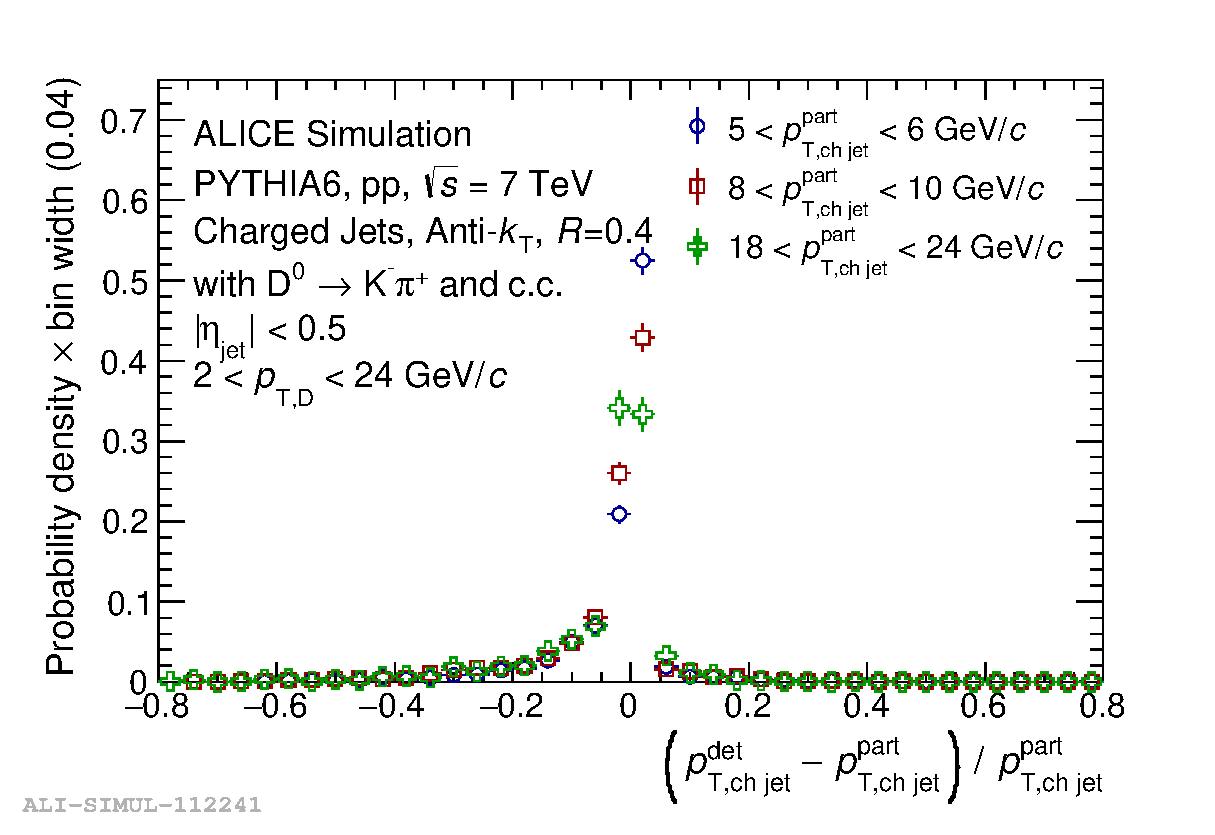
\includegraphics[width=\textwidth]{img/HQ16_Simulation_DetectorResponse}
\caption{\label{fig:HQ16_Simulation_DetectorResponse} Probability density distribution of the jet momentum shift, for ranges of \ptchjet.}
\end{minipage}\hspace{1pc}%
\begin{minipage}{.48\textwidth}
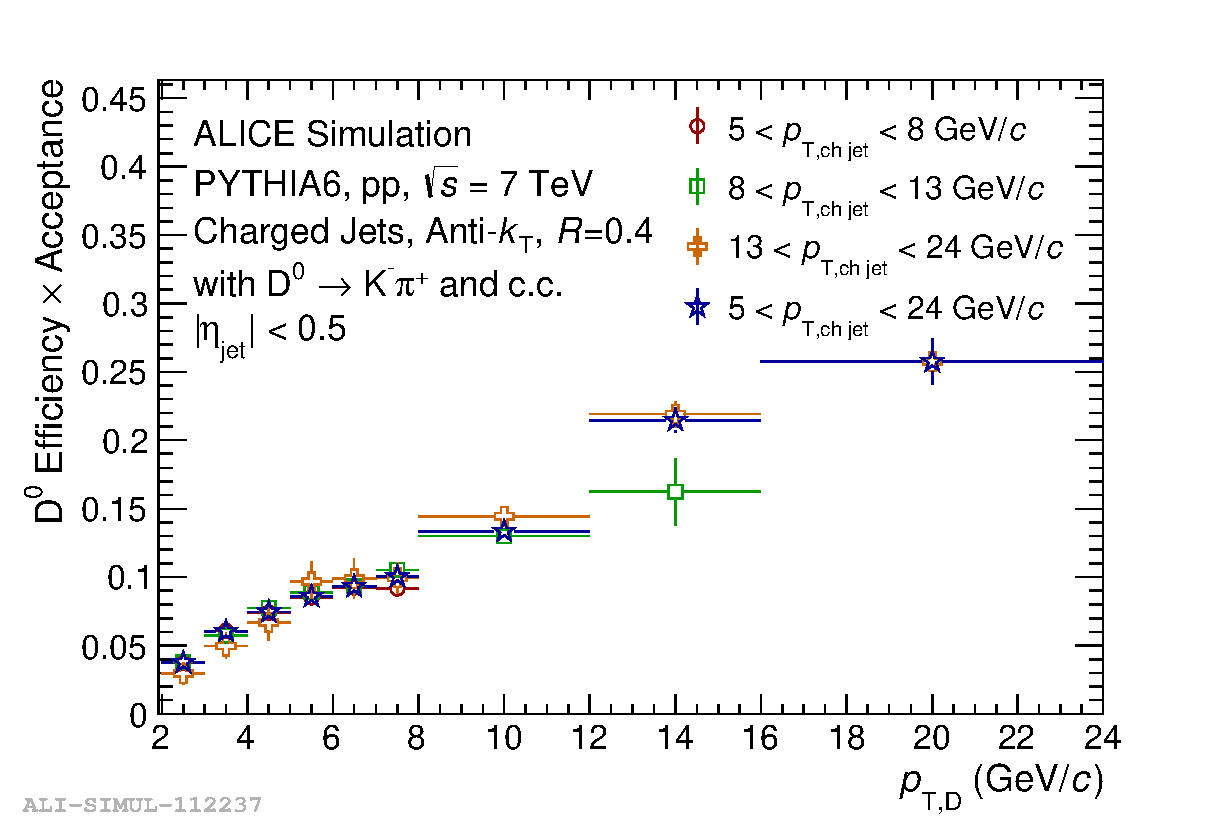
\includegraphics[width=\textwidth]{img/HQ16_Simulation_EfficiencyVsDPt}
\caption{\label{fig:HQ16_Simulation_EfficiencyVsDPt}Efficiency~$\times$~Acceptance of \Dzero\ mesons vs. \ptd\ for ranges of \ptchjet.}
\end{minipage} 
\end{figure}

The detector performance was assessed using the charm-enhanced MC production. 
Reconstructed detector-level D-tagged jets are matched with their corresponding counterparts at generator-level and the variable
%\begin{equation}
$\sigma_{\ptchjet}=\left( \ptchjetdet - \ptchjetgen \right) / \ptchjetgen$,
%\label{eq:energyshift}
%\end{equation}
is computed,
where \ptchjetdet\ and \ptchjetgen\ are the transverse momenta of the D-tagged jet at detector-level and at generator-level, respectively.
Its probability density distribution is shown in Fig.~\ref{fig:HQ16_Simulation_DetectorResponse} for three ranges of \ptchjetgen. No significant dependence on \ptchjetgen\ is observed.
The shape of the distribution features a sharp peak at zero and is skewed towards negative values, due to tracking inefficiency (higher probability of
reconstructing smaller jet momenta than the generated ones). The jet momentum resolution (standard deviation of $\sigma_{\ptchjet}$) for \Dzero-tagged jets is approximately \mbox{$11$\%}, 
slightly smaller with respect to its value for inclusive jets~\cite{ALICE:2015e}. The mean jet momentum shift is approximately \mbox{$-3$\%}.
The reconstruction efficiency is calculated as the ratio of the yield of reconstructed D-tagged jets over all generated D-tagged jets, as a function of generator-level observables.
It is shown in Fig.~\ref{fig:HQ16_Simulation_EfficiencyVsDPt} as a function of \ptd\ for different ranges of \ptchjet; it shows a stark dependence on \ptd, mainly due to
varying topological cuts. No significant dependence on \ptchjet\ is observed in the range $5<\ptchjet<24$~\GeVc.

\begin{figure}[tb]
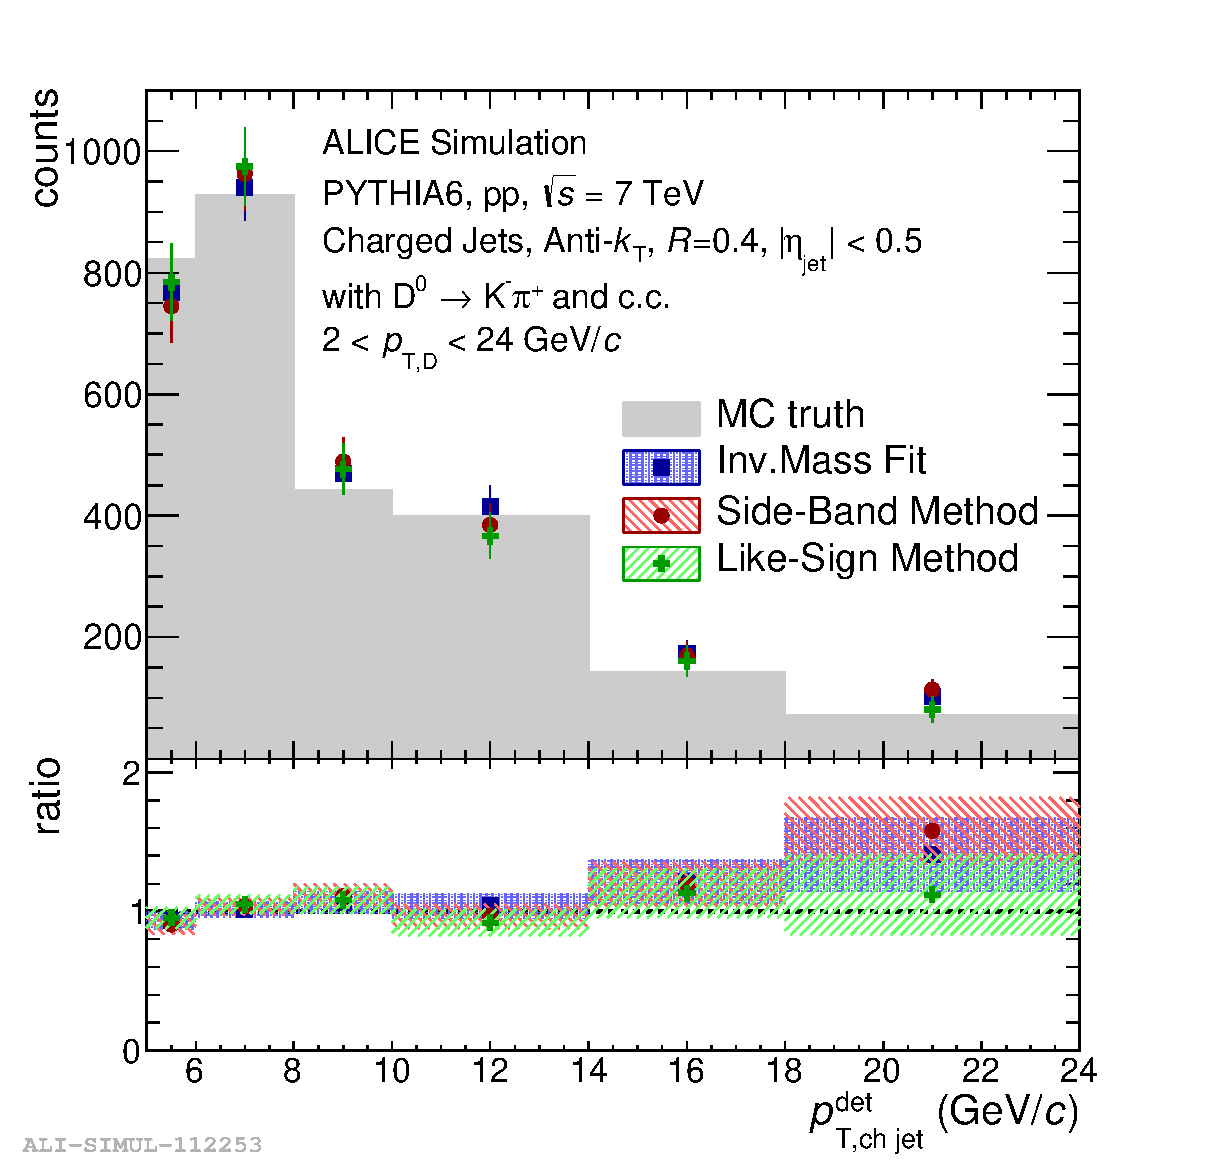
\includegraphics[width=.50\textwidth]{img/HQ16_Simulation_MethodComparison}\hspace{1pc}%
\begin{minipage}[b]{.50\textwidth}\caption{\label{fig:HQ16_Simulation_MethodComparison}\Dzero-jet signal yield extracted using the invariant mass fit (blue squares), side-band method (red circles) and like-sign method (green triangles)
compared with the MC truth (gray filled area). The bottom panel shows the ratio to the MC truth. The yields are corrected for the reconstruction efficiency but not for distortions due to detector jet-momentum resolution.}
\end{minipage}
\end{figure}

The minimum-bias production was used to validate the invariant mass analysis. 
Figure~\ref{fig:HQ16_Simulation_MethodComparison} shows the D-tagged jet yields as a function of \ptchjetdet\ obtained using the invariant mass fit, 
side-band and like-sign methods, compared to the MC truth. All signal extraction methods perform well and do not show significant biases, beyond the statistical uncertainties assigned to each.

\section{Conclusions}
ALICE has a great potential for measuring jets with charm content tagged using reconstructed D mesons.
%in pp collisions, especially at low momentum ($\ptchjet \lesssim 30$~\GeVc) with the data collected at $\s=7$~TeV,
%as well as the intermediate jet momentum ($\ptjet\approx100$~\GeVc) and
%low D-meson momentum by exploiting the data collected at $\s=8,\,13$~TeV with the calorimeter triggers.
%In \PbPb\ and \pPb\ collisions ALICE will study cold and hot nuclear matter effects
%looking at the yields and fragmentation functions of \Dzero-tagged jets.
The ALICE detector performance for \Dzero-tagged jets was assessed using MC simulations
for pp collisions at $\s=7$~TeV. The \Dzero-jet momentum resolution was measured to be about 11\%; the reconstruction efficiency, independent of \ptchjet, ranges from 5\% to 25\% as a function of \ptd.
Three methods were implemented to extract the signal: invariant mass fit, side-band and like-sign subtraction.
The three methods were validated using a MC simulation and do not show biases larger than the statistical uncertainties.

\section*{References}
\bibliography{biblio}{}
\bibliographystyle{iopart-num}

\end{document}


